\hypertarget{stm32f4xx__hal__rcc_8c}{}\section{Dokumentacja pliku S\+T\+M/\+W\+D\+S\+\_\+\+Kosc\+\_\+\+Linux/\+Drivers/\+S\+T\+M32\+F4xx\+\_\+\+H\+A\+L\+\_\+\+Driver/\+Src/stm32f4xx\+\_\+hal\+\_\+rcc.c}
\label{stm32f4xx__hal__rcc_8c}\index{S\+T\+M/\+W\+D\+S\+\_\+\+Kosc\+\_\+\+Linux/\+Drivers/\+S\+T\+M32\+F4xx\+\_\+\+H\+A\+L\+\_\+\+Driver/\+Src/stm32f4xx\+\_\+hal\+\_\+rcc.\+c@{S\+T\+M/\+W\+D\+S\+\_\+\+Kosc\+\_\+\+Linux/\+Drivers/\+S\+T\+M32\+F4xx\+\_\+\+H\+A\+L\+\_\+\+Driver/\+Src/stm32f4xx\+\_\+hal\+\_\+rcc.\+c}}


R\+CC H\+AL module driver. This file provides firmware functions to manage the following functionalities of the Reset and Clock Control (R\+CC) peripheral\+:  


{\ttfamily \#include \char`\"{}stm32f4xx\+\_\+hal.\+h\char`\"{}}\newline
Wykres zależności załączania dla stm32f4xx\+\_\+hal\+\_\+rcc.\+c\+:\nopagebreak
\begin{figure}[H]
\begin{center}
\leavevmode
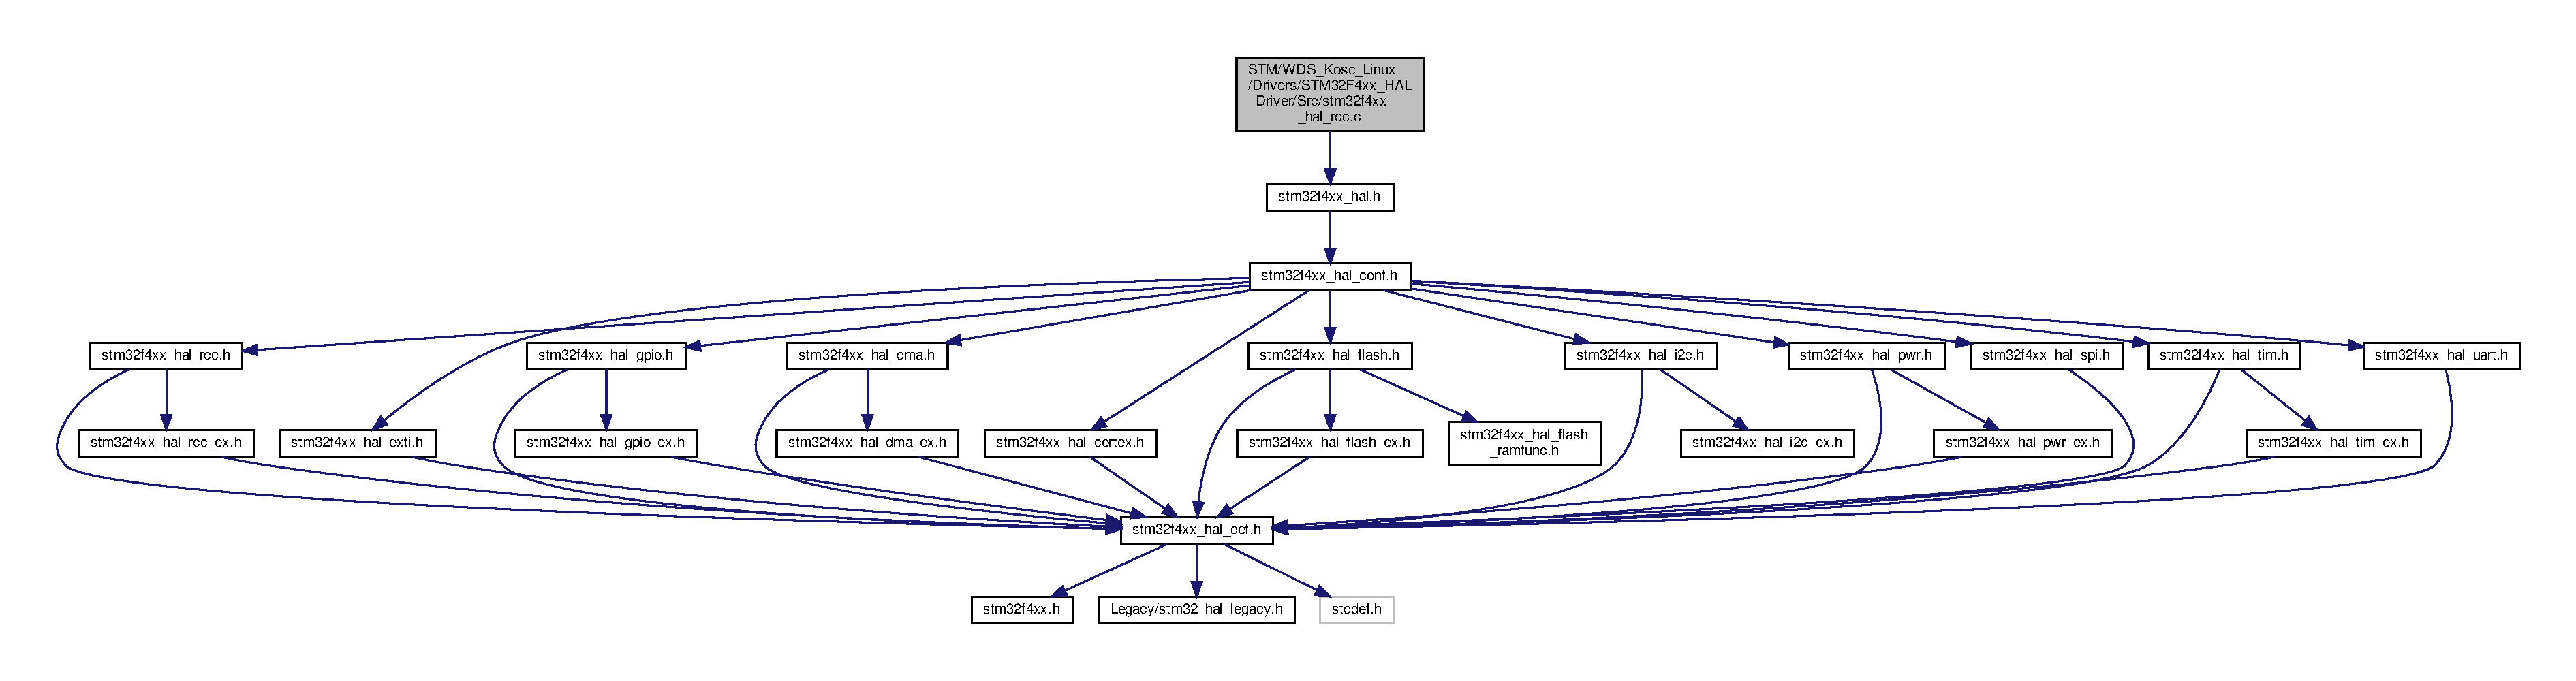
\includegraphics[width=350pt]{stm32f4xx__hal__rcc_8c__incl}
\end{center}
\end{figure}


\subsection{Opis szczegółowy}
R\+CC H\+AL module driver. This file provides firmware functions to manage the following functionalities of the Reset and Clock Control (R\+CC) peripheral\+: 

\begin{DoxyAuthor}{Autor}
M\+CD Application Team
\begin{DoxyItemize}
\item Initialization and de-\/initialization functions
\item Peripheral Control functions
\end{DoxyItemize}
\end{DoxyAuthor}
\begin{DoxyVerb}==============================================================================
                    ##### RCC specific features #####
==============================================================================
  [..]
    After reset the device is running from Internal High Speed oscillator
    (HSI 16MHz) with Flash 0 wait state, Flash prefetch buffer, D-Cache
    and I-Cache are disabled, and all peripherals are off except internal
    SRAM, Flash and JTAG.
    (+) There is no prescaler on High speed (AHB) and Low speed (APB) busses;
        all peripherals mapped on these busses are running at HSI speed.
    (+) The clock for all peripherals is switched off, except the SRAM and FLASH.
    (+) All GPIOs are in input floating state, except the JTAG pins which
        are assigned to be used for debug purpose.

  [..]
    Once the device started from reset, the user application has to:
    (+) Configure the clock source to be used to drive the System clock
        (if the application needs higher frequency/performance)
    (+) Configure the System clock frequency and Flash settings
    (+) Configure the AHB and APB busses prescalers
    (+) Enable the clock for the peripheral(s) to be used
    (+) Configure the clock source(s) for peripherals which clocks are not
        derived from the System clock (I2S, RTC, ADC, USB OTG FS/SDIO/RNG)

                    ##### RCC Limitations #####
==============================================================================
  [..]
    A delay between an RCC peripheral clock enable and the effective peripheral
    enabling should be taken into account in order to manage the peripheral read/write
    from/to registers.
    (+) This delay depends on the peripheral mapping.
    (+) If peripheral is mapped on AHB: the delay is 2 AHB clock cycle
        after the clock enable bit is set on the hardware register
    (+) If peripheral is mapped on APB: the delay is 2 APB clock cycle
        after the clock enable bit is set on the hardware register

  [..]
    Implemented Workaround:
    (+) For AHB & APB peripherals, a dummy read to the peripheral register has been
        inserted in each __HAL_RCC_PPP_CLK_ENABLE() macro.\end{DoxyVerb}


\begin{DoxyAttention}{Uwaga}

\end{DoxyAttention}
\subsubsection*{\begin{center}\copyright{} Copyright (c) 2017 S\+T\+Microelectronics. All rights reserved.\end{center} }

This software component is licensed by ST under B\+SD 3-\/\+Clause license, the \char`\"{}\+License\char`\"{}; You may not use this file except in compliance with the License. You may obtain a copy of the License at\+: opensource.\+org/licenses/\+B\+S\+D-\/3-\/\+Clause 